\section{Introduzione}
Lo scopo di questo progetto consiste nella classificazione dell'attività fisica svolta da un individuo grazie a delle misure ottenute con una board Arduino Nano 33 BLE Sense posizionata sopra la caviglia di un soggetto. Dopo essersi connessi alla board tramite BLE e in base al firmware caricato sull'Arduino, è possibile utilizzare l'applicazione in due modalità:
\begin{itemize}
	\item modalità acquisizione dati: l'applicazione riceve e salva i dati inviati dalla piattaforma;
	\item modalità activity tracker: l'applicazione visualizza la predizione dell'attività che il soggetto sta svolgendo (camminata, cyclette, salto con la corda oppure l'individuo è fermo).
\end{itemize}
Sono stati utilizzati i seguenti sensori presenti sulla board:
\begin{itemize}
	\item accelerometro triassiale;
	\item giroscopio triassiale;
	\item sensore di temperatura e di umidità.
\end{itemize}
Tuttavia, i dati di temperatura e umidità non sono stati utilizzati poiché i dati ricavati non si sono mostrati essere significativi per l'obiettivo di questo progetto.

Per l'attività di classificazione dell'attività si è scelto di utilizzare un approccio \textit{black-box}, utilizzando una rete neurale opportunamente allenata con i dati raccolti dalla board. La rete neurale, sviluppata tramite il framework Edge Impulse, è stata poi installata sull'Arduino. Utilizzando quindi un modello di \textit{edge computing}, è stato possibile realizzare una applicazione, sviluppata grazie al framework Qt, che si occupa solamente della visualizzazione dei dati e della predizione dell'attività svolta. In questo modo, si è potuto mantenere una frequenza di campionamento dei dati relativamente alta (circa \SI{66}{\hertz}) senza sovraccaricare la comunicazione BLE.

\section{Acquisizione dei dati}
Per poter acquisire i dati con Arduino, è stato necessario sviluppare un firmware apposito che consentisse di eseguire le acquisizioni utilizzando la tecnologia Bluetooth Low Energy (BLE), in cui è stato utilizzato Arduino come \textit{Peripheral}, che trasmette i dati sotto forma di caratteristiche, e l'applicazione come \textit{Central}, che li riceve.

I dati acquisiti con il BLE, come preannunciato nella sezione precedente, sono: le accelerazioni e le velocità di rotazione entrambe sui tre assi, la temperatura e l'umidità.

Nelle prime acquisizioni delle misure sono stati riscontrati due problemi: il primo riguarda il fatto che il delay tra coppie di misure successive non corrisponde sempre all'incirca a \SI{15}{\milli\second} (come desiderato) a causa del collegamento BLE, che provoca perdite di tempo; mentre il secondo è relativo alle perdite di campioni  misurati durante l'invio delle misure tramite il BLE. Per questi due motivi all'interno del firmware è stato creato un buffer circolare in modo da poter bufferizzare le acquisizioni da trasmettere nel Bluetooth. In conseguenza a questa modifica si è visto che il delay tra coppie di misure assume sempre valori prossimi a \SI{15}{\milli\second} e soprattutto che non vengono perse delle acquisizioni perchè vengono mantenute nel buffer.

\todo{inserire anche mutex? + nuove modifiche}

\todo{mancano dei problemi?}

\section{Edge Impulse}
\todo{I dati acquisisti sono stati caricati su Edge Impulse. Come è stato creato l'impulse. Su cosa lavora. Cosa produce edge impulse. Come son state modificate le finestre. Feature spettrali. Bontà del modello e testing.}

\section{Classificazione delle attività}
Per realizzare la classificazione e poi visualizzarla sull'applicazione è stato sviluppato un ulteriore firmware, al cui interno sono stati creati due thread differenti. Nel primo vengono acquisiti i dati dai sensori fino a quando il buffer non risulta pieno, mentre nel secondo si aggiorna il collegamento BLE in modo da poter trasmettere successivamente la previsione della classificazione. Una volta che il buffer è pieno si estraggono i suoi elementi tramite Digital Signal Processing in modo da convertire il buffer in un segnale, che viene poi passato al classificatore per fare inferenza. La realizzazione concreta della classificazione prevede di richiamare le librerie di Edge Impulse. Infine il risultato della classificazione viene trasmesso tramite una caratteristica su BLE all'applicazione, che mostra a video l'immagine relativa all'attività fisica rilevata. Le possibili schermate visualizzate sull'applicazione si distinguono in base all'attività come mostrato nella figura \ref{fig:attivitafisica}.

\begin{figure}[tbh]
	\centering
	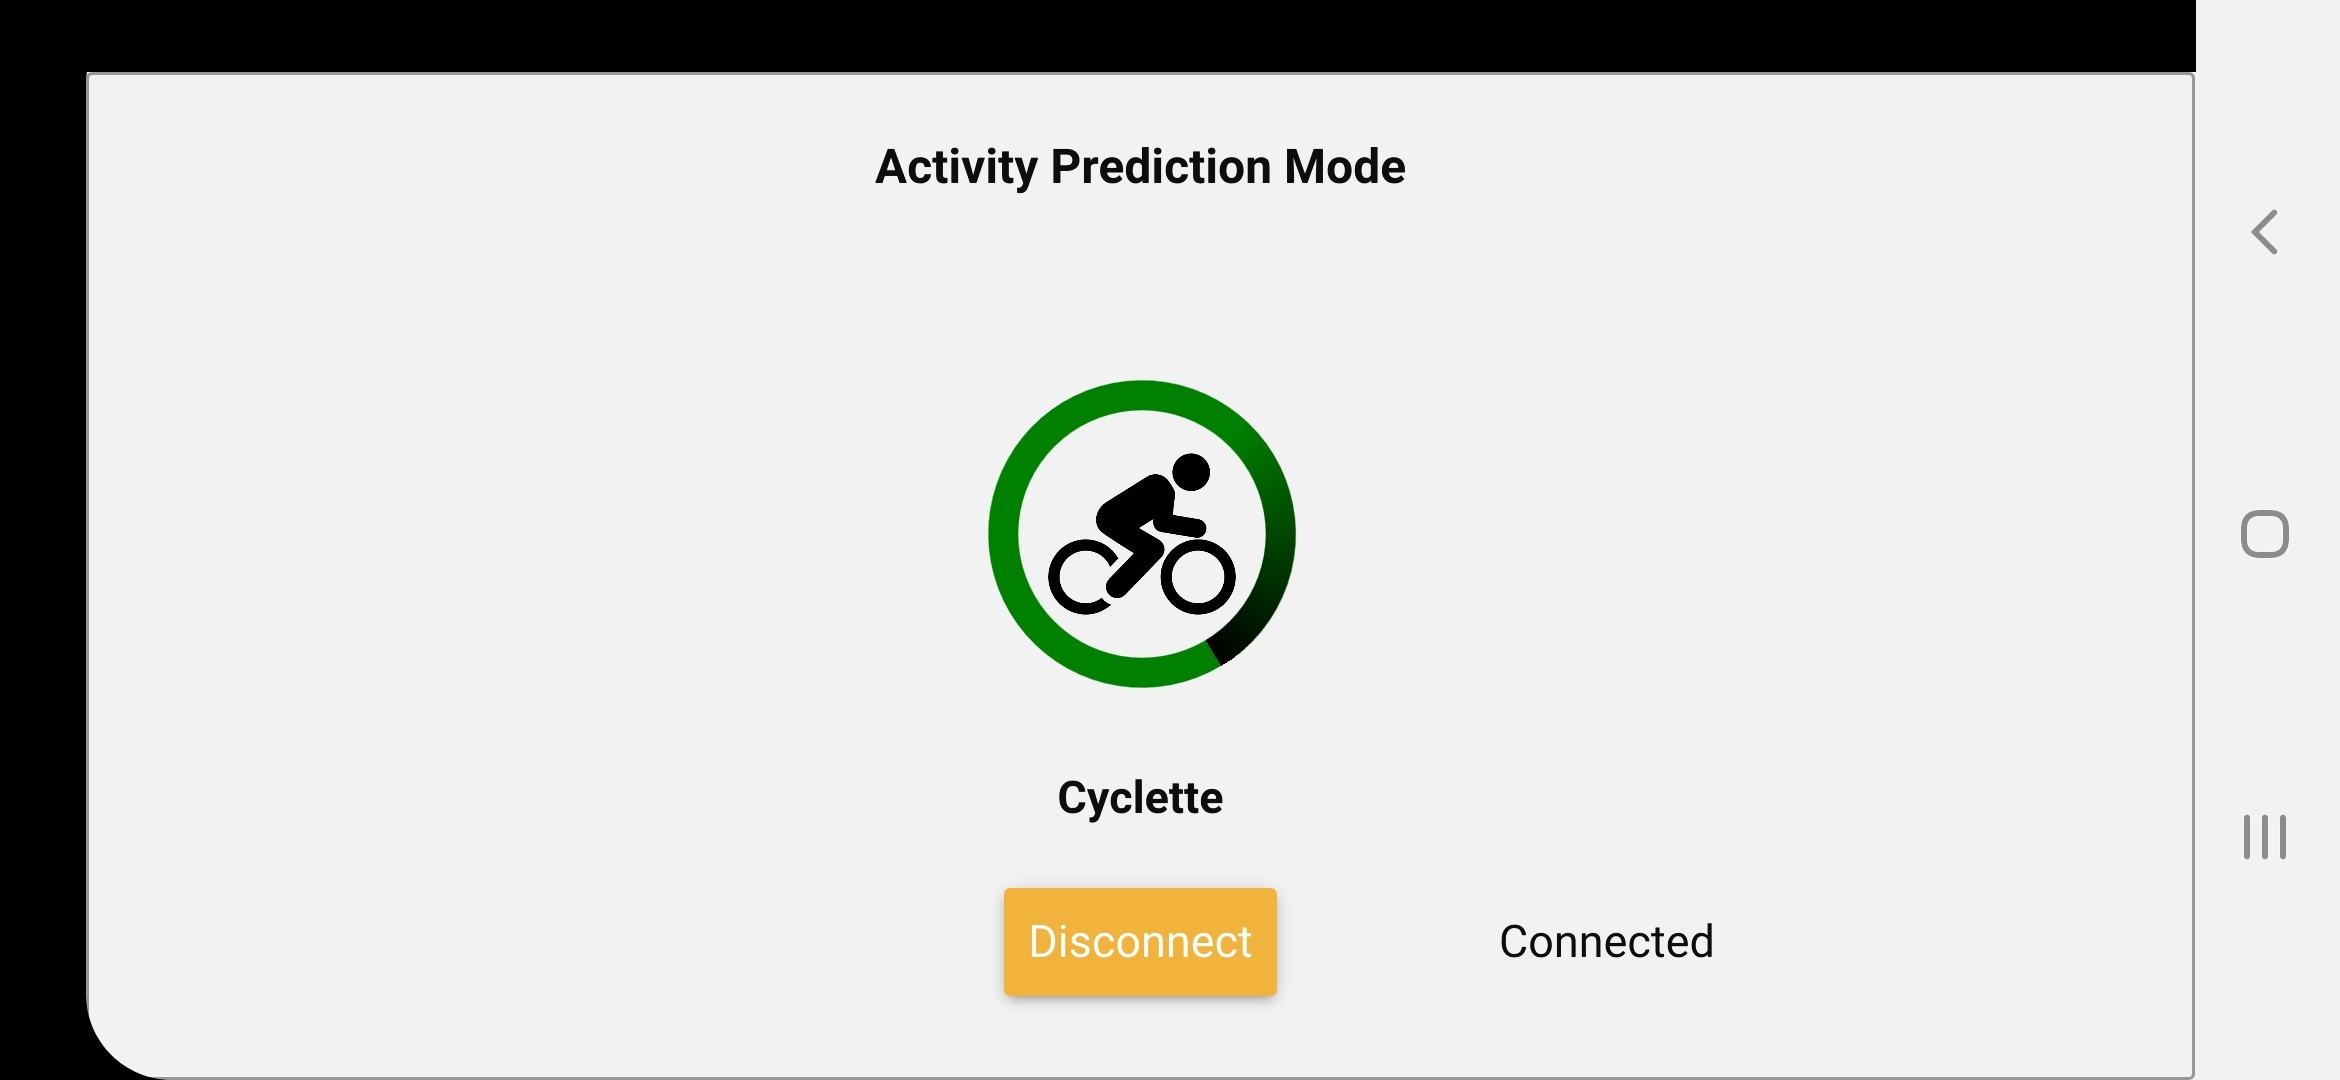
\includegraphics[width=0.4\linewidth]{./ImageFiles/cyclette}
	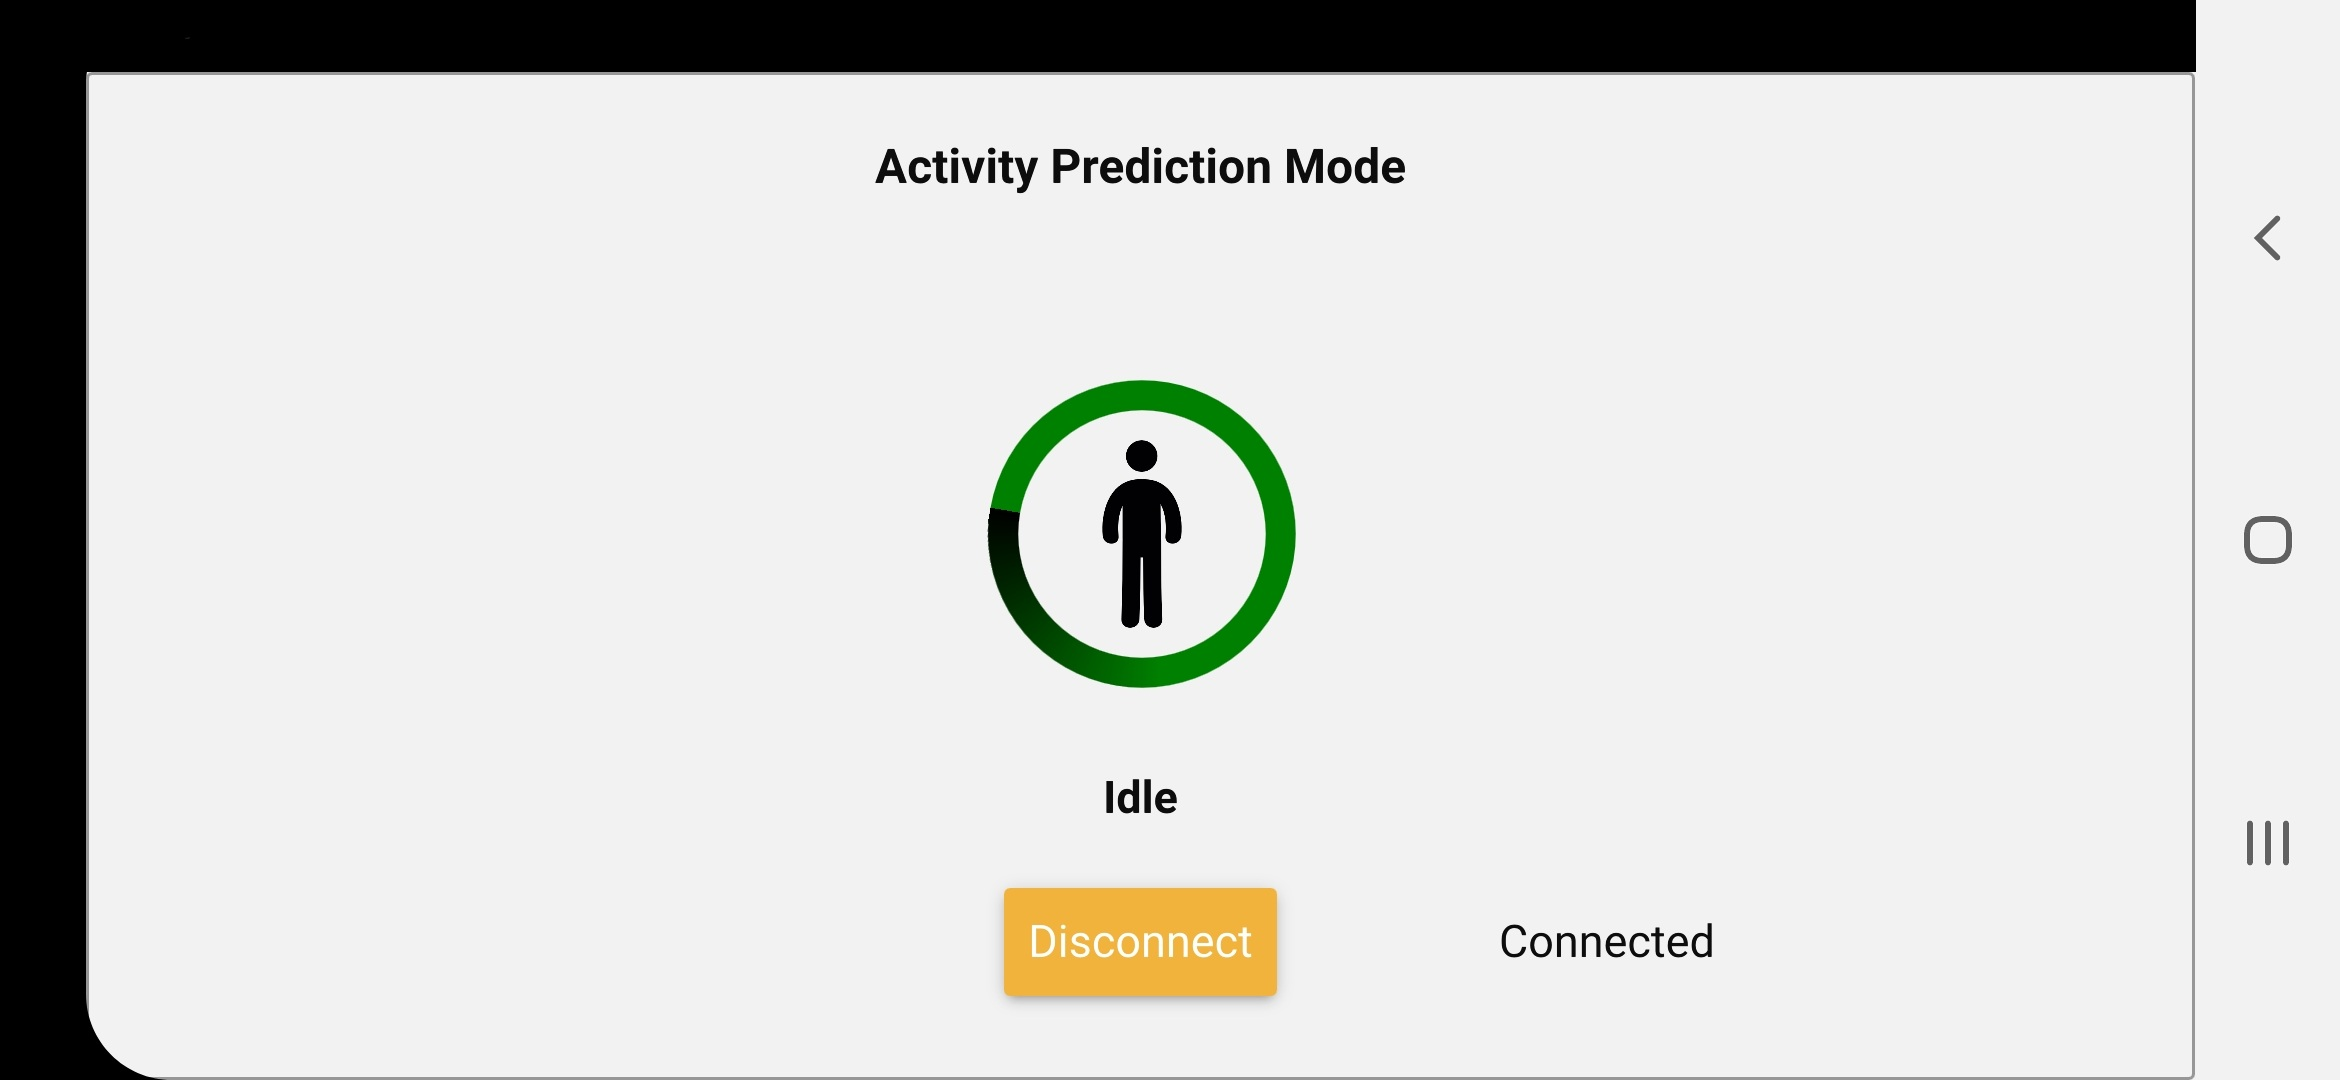
\includegraphics[width=0.4\linewidth]{./ImageFiles/idle}
	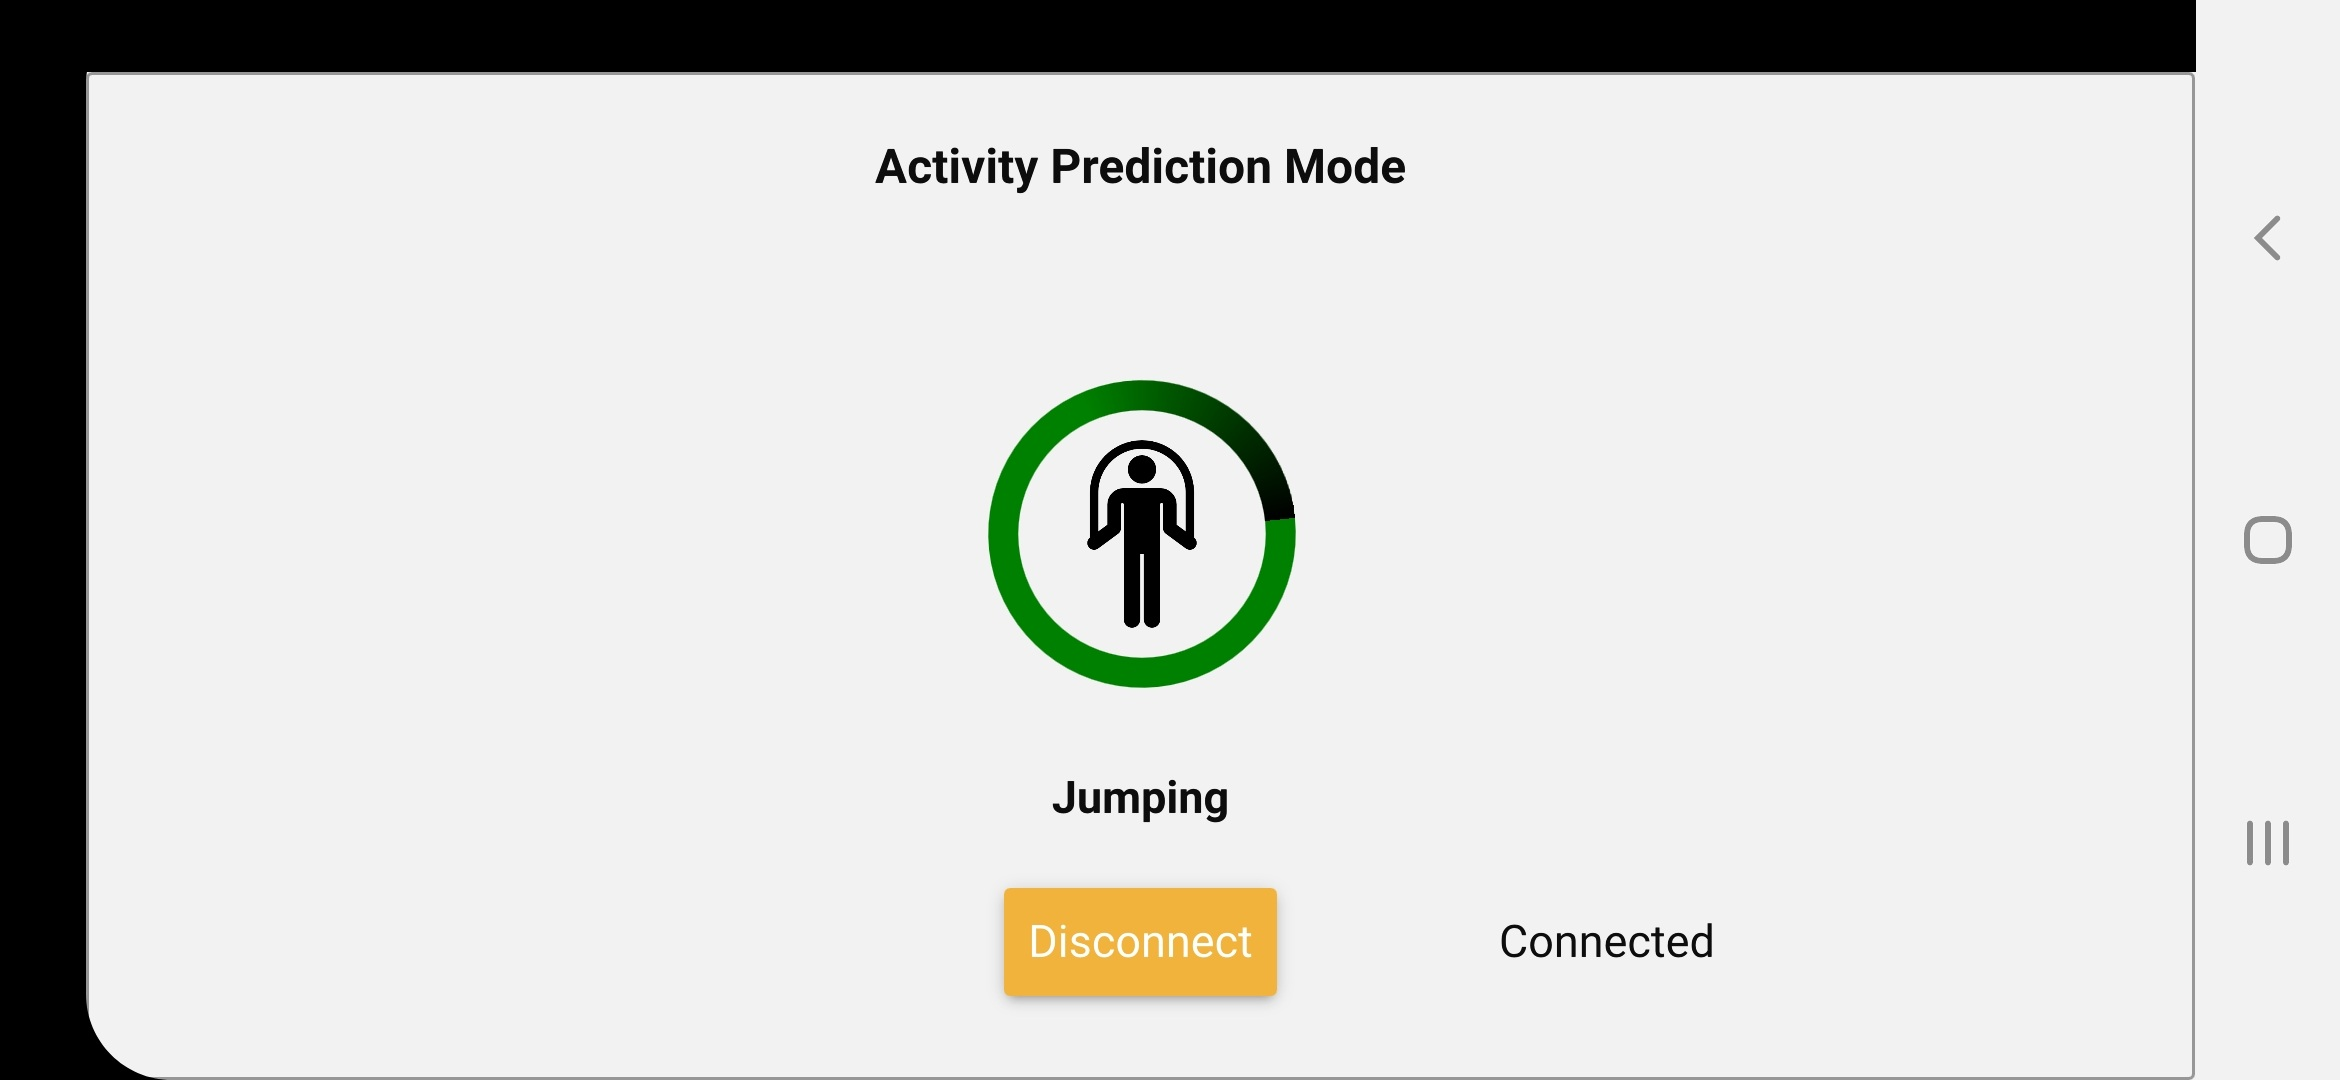
\includegraphics[width=0.4\linewidth]{./ImageFiles/jumping}
	%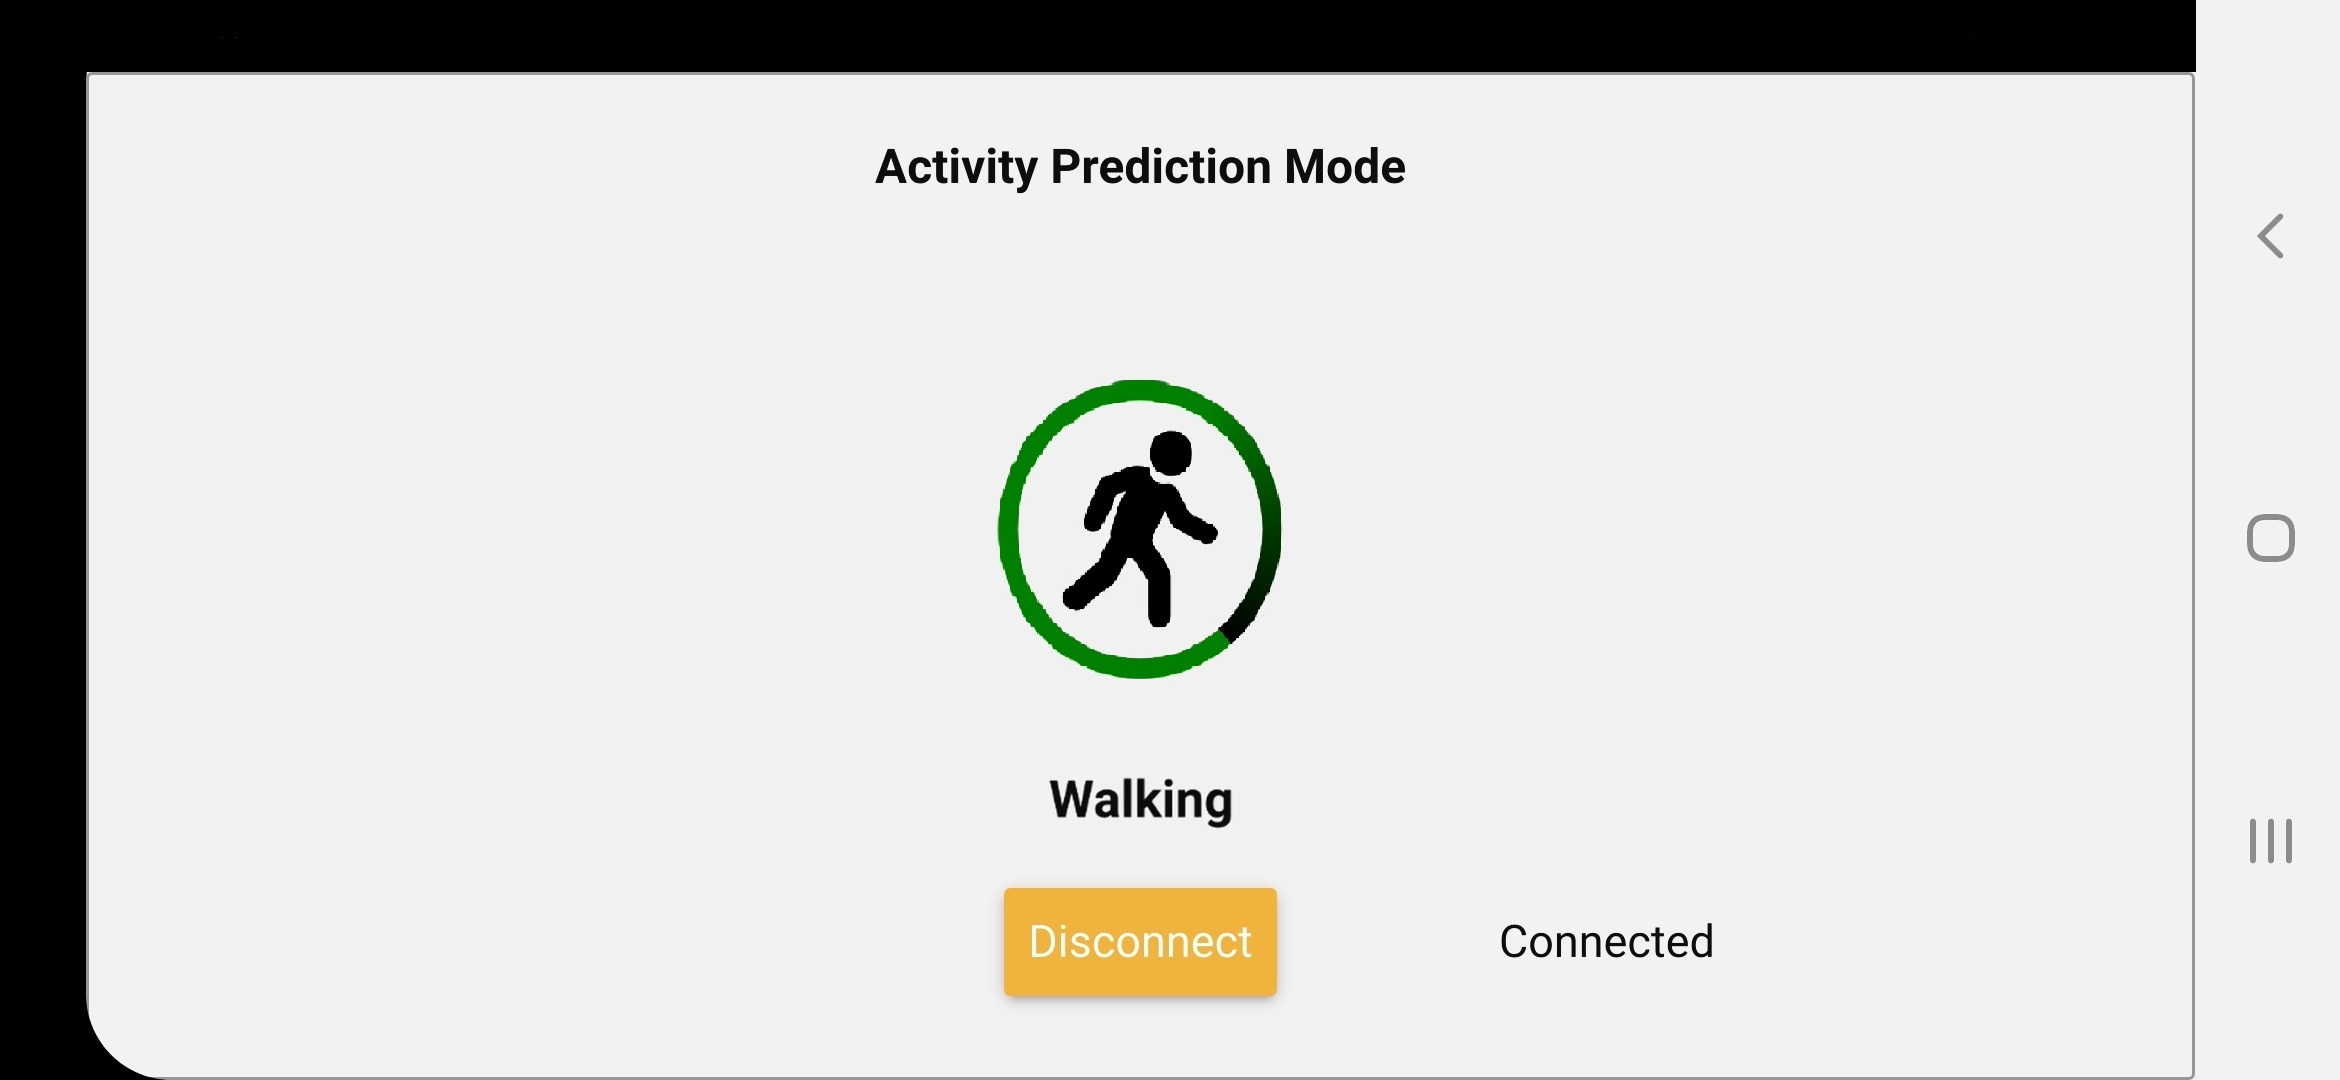
\includegraphics[width=0.4\linewidth]{./ImageFiles/walking}
	\caption{Schermate per le possibili attività: cyclette, fermo, salto della corda e camminata.}
	\label{fig:attivitafisica}
\end{figure}
\todo{manca schermata walking}

Invece nei momenti in cui non si riesce a classificare l'attività in corso in nessuna di quelle possibili si visualizza la schermata della figura \ref{fig:attesa}.

\begin{figure}[tbh]
	\centering
	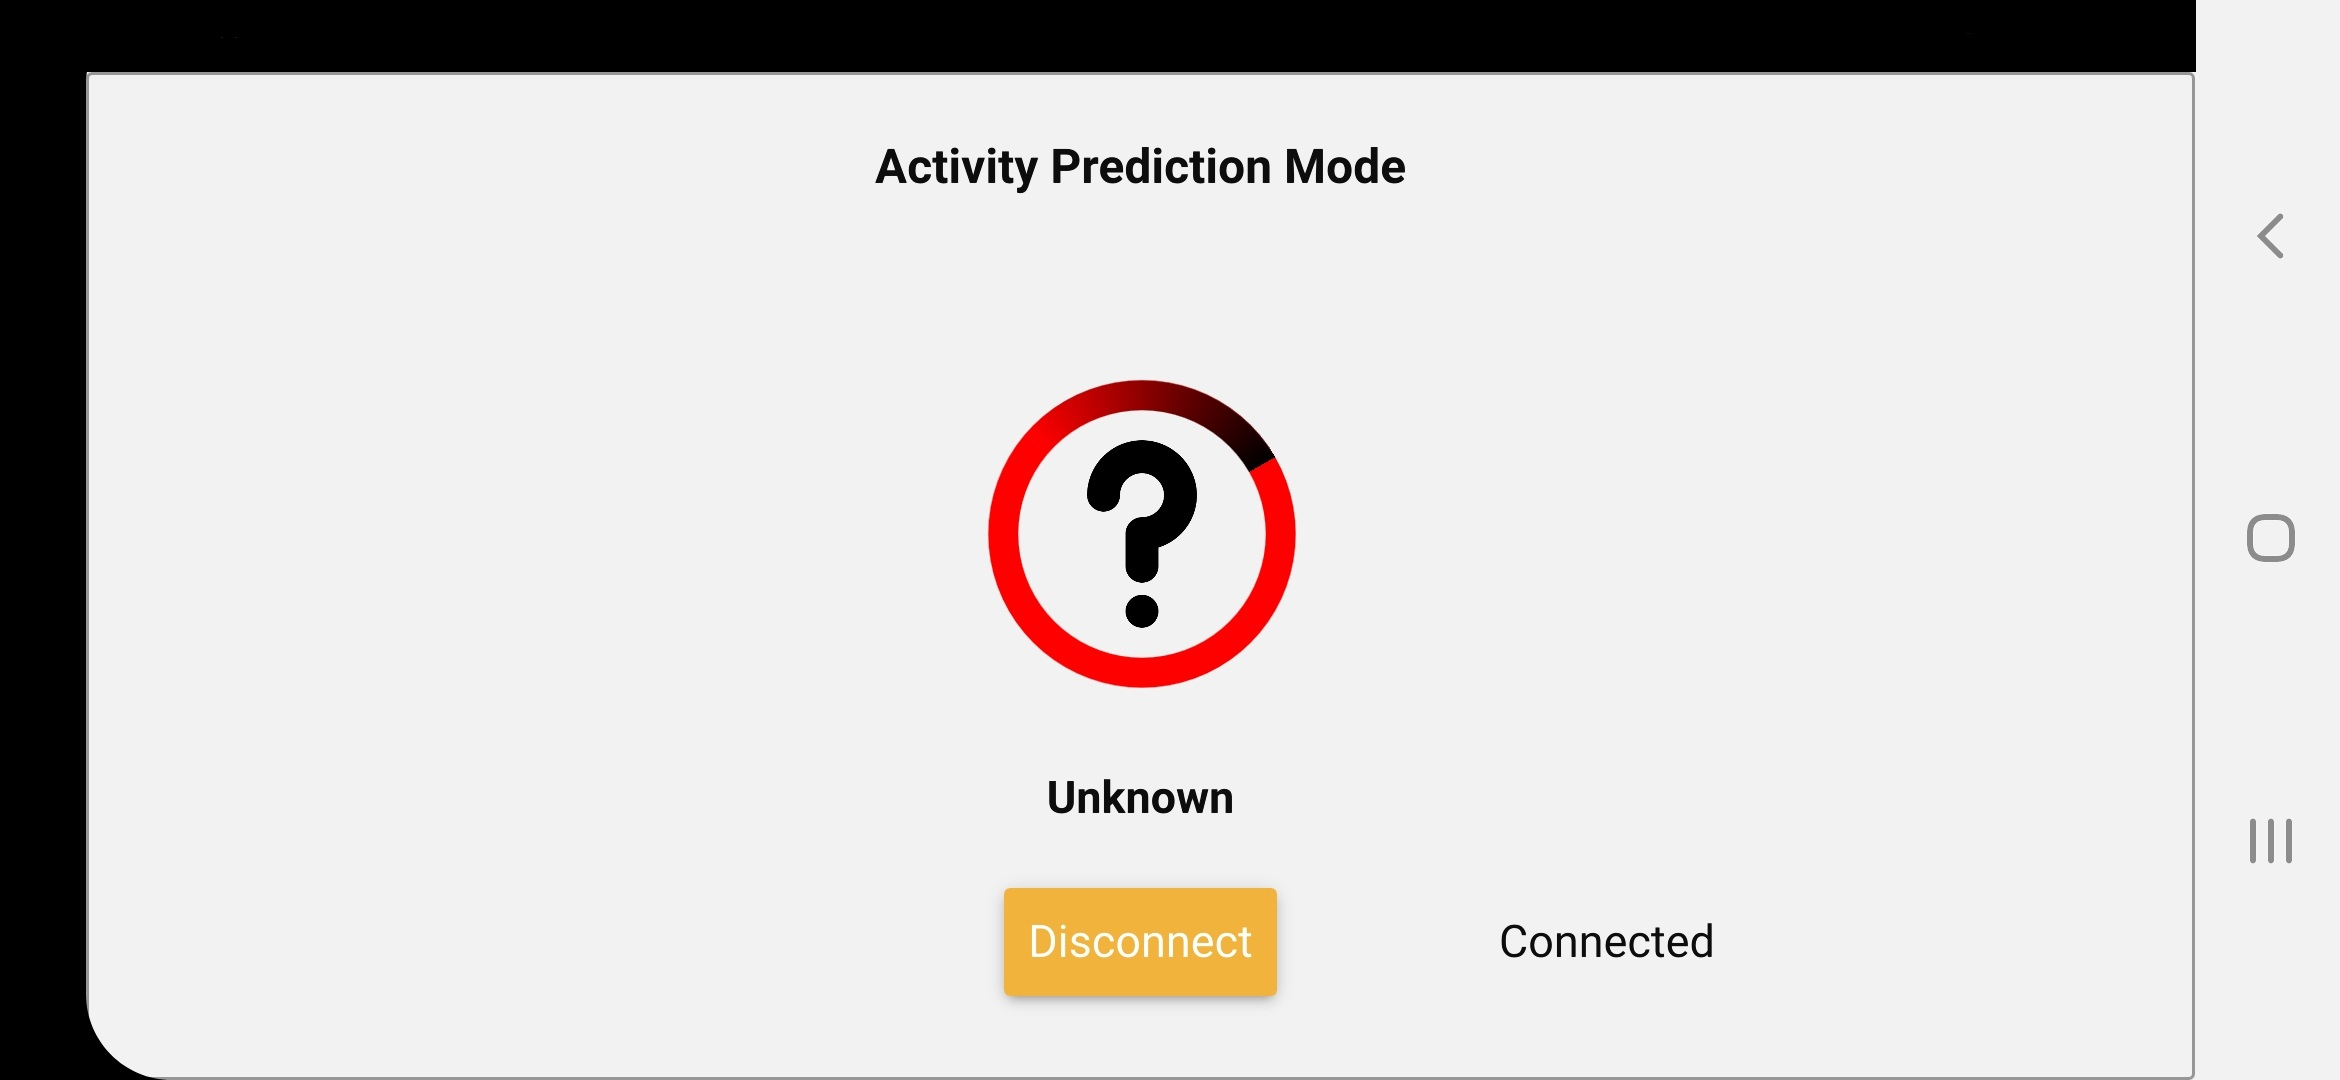
\includegraphics[width=0.4\linewidth]{./ImageFiles/unknown}
	\caption{Schermata per le attese precedenti la classificazione o per misure non classificabili.}
	\label{fig:attesa}
\end{figure}

\todo{Quali sono i tempi che impiega il firmware. Per passare da una attività all'altra servono circa tot secondi perchè si deve svuotare il buffer.}